
         %%%%%%%%%%%%%%%%%   PROOFS   %%%%%%%%%%%%%%%%%%%%
\chapter{Introduction to Proofs}
For those who are already comfortable writing formal arguments and mathematical proofs, this chapter can be skipped. But many students approach the subject of proofs with trepidation and this chapter is included to connect the prior subject of formal logic and all the chapters that follow which develop their material with more formal presentations including proofs. 

To introduce proofs we will depend upon a few formal definitions that you learned in high school and prove some other properties using those definitions. 

\begin{definition}[Even and Odd Integers]
An even integer is one that is equal to twice some other integer. An odd integer is one that is equal to twice some other integer plus 1.
\end{definition}

But we must reiterate this text is not designed to teach but to provide a  support to the learning and later reference to the material within our scope. This is seen here in that other than a few examples needed to briefly illustrate some points, one will never learn to prove anything from this chapter. Instead it is a brief survey of basic terminology and cartoons of essential arguments to quickly remind the reader how to structure a proof of that type. We make some attempt in later chapters to give specific examples of the more interesting ways we reason about material using some of the techniques we present in its cartoon form in this chapter.

\section {Inference}
   \subsection {Valid Arguments in Propositional Logic}
\begin{definition}[Argument]
We define an \textit{argument} as some series of statements meant to convince the reader of the truth of some proposition we call the \textit{conclusion}.
\end{definition}

 
   \subsection {Rules of Inference for Propositional Logic}
We already saw how we can show the logical equivalence of two compound propositions using truth tables. However this becomes impractical as the number of atomic propositions grows. It also becomes difficult to follow the argument if this is the only way used to demonstrate the logical equivalence. In a high school geometry course you have already seen a different way that depends upon a series of statements and certain established rules of inference. We show how these are built from the logic.

One of the most basic is represented by this equivalence:
$$p \land (p \rightarrow q) \equiv q$$
This statement can be read as "Given that p is true with the the conditional statement if p is true that q must be true then it is logically equivalent to the value of q." When you construct the truth table you see this logical equivalence. This essential point of logic is called Modus Ponens, which is short for the Latin phrase "\textit{modus ponendo ponens}" which means "mode that affirms by affirming" and goes back to antiquity. It is also called the law of detachment. In more advanced material on logic this is considered beyond the logic presented up to now but we are not going to let that detail trouble us. It is the first of many argument forms that are used in argumentation. 

In antiquity logic came from rhetoric and the recognition that it was the rhetorical form that sometimes gave the truth or falsity of an argument and not the meaning of the propositions. That is why we jumped over natural language and the translations back and forth between symbolic logic and natural language. While an argument may sound persuasive, sometimes when reduced to its symbolic equivalent we can find a flaw in the argument.

The first thing you will notice is that this presentation of these rules of valid argumentation, or rules of inference, are not laid out like the compound propositions we saw before. In fact they are laid out in a way that mimics natural language by mimicing a sentence structure. For example I can state modus ponens in words as:\\
It is the case that whenever p is true that q is also true\\
It is the case that p is true\\
Therefore it is the case that q must be true. \\

It is customary to place a horizontal rule between the argument and the conclusion which is stated following the word, "therefore". Mathematicians have a symbol to mean therefore which is $\therefore$  . 

   \begin{table}[htbp]
   \centering
   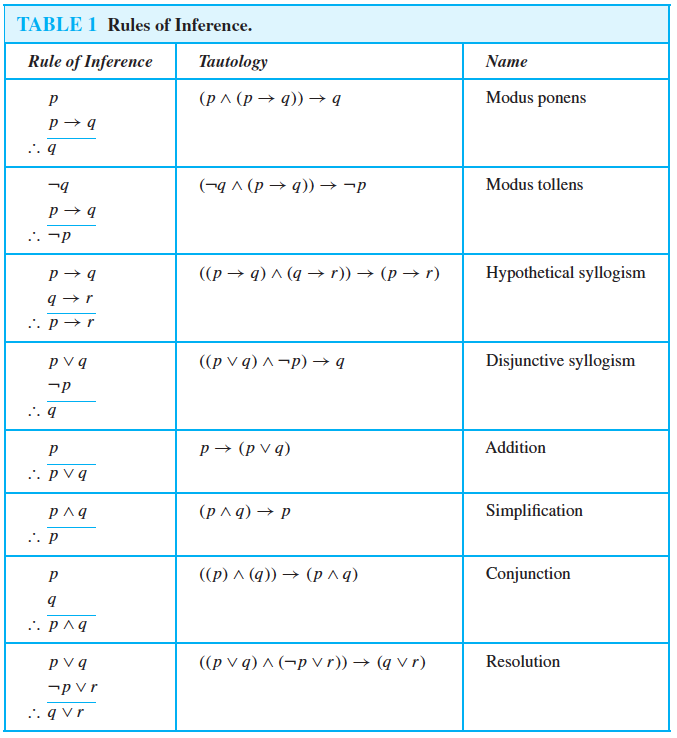
\includegraphics [width=5in] {Table-1-6-1-RulesOfInference}
   \caption{Common Rules of Inference}
   \label{table:rulesofinference}
   \end{table}

   \subsection {Using Rules of Inference to Build Arguments}
\begin{definition}[Argument Form]\index{argument form}
An argument in propositional logic is a sequence of propositions. All but the final proposition in the argument are called premises and the final proposition is called the conclusion. An argument is valid if the truth of all its premises implies that the conclusion is true.

An argument form in proposition logic is a sequence of compoutn propositions involving propositional variables. An arguent form is valid if no matter which particular propositions are substituted for the proposition variables in its premise, th econclusion is true if the premises are all true. (valid v sound??)
\end{definition}


If you look you will note that a great many properties in mathematics are stated as either conditional or bi-conditonal statements. "If $i$ is an even integer, then $i+1$ is an odd integer." If you want to mount an argument as to why this assertion must be true, you must demonstrate a series of equivalent statements that cannot be refuted until you reach the conclusion. In this case you will already have some definitions or other propositions that are not refuted, in this case the definiton of what it means to be even or odd. You must then offer the next assertion and be prepared to defend it. For example, "well if $i$ is an even integer then there is some other integer which I'll call $k$ such that $i=2k$ by the definition of what it means to be an even integer." Note that I have given both a new assertion, "there is some integer $k$ such that $i=2k$" and a justification, "\dots by the definition of what it means to be an even integer." In a classic two column presentation of the argument you would have one column which has the assert and another which has the justification for that assertion. You may have been taught this form in your high school geometry class. It helps you when you are first learning this style of formal argumentation since it forces you to support your argument (and makes grading so much easier!!!). Continuing our example, my next statement can be "$i+1=2k+1$, equals plus equals gives equals." We then can observe that "$2k+1$ is odd, by the definition of odd." Finally we conclude with "Therefore $i+1$ is an odd integer since it is equal to $2k+1$" and we have now completed the argument. A classic flourish in the presentation of such an argument is to put Q.E.D. which is the abbreviation for \textit{Quod Erat Demonstrandum}, a Latin phrase that means "that which was to be demonstrated." In textbooks this is often replace with a blackened or open square to signify that we reached the conclusion and the argument is over ($\blacksquare$ or $\square$). typographicallycalled a tombstone or Halmos.

Formal arguments like this are called proofs.

Note an important logical point about the prior argument. We claim it is application of the modus ponens inference. But where is the truth of the antecedent? Reconsider the implication, if $p$ then $q$. We already know that when the antecedent is false we evaluate the implication as true. That is to say in the last example that if it is the case that $i$ is NOT an even integer, that we make no claim about $i+1$. Once you ignore the two cases where the antecedent is false you only have two cases where it is true. For the conditional statement to be true we must argue that the case where the consequent is true is necessarily true and that the consequent must necessarily never be false. This allows us to accept the antecedent as true since we are only interested in conditionals with a true antecedent. If this does not make sense on the first reading, don't fret. But sooner or later it will occur to you that many conditional statements apply modus ponens without dealing with false antecedents. 

You will rarely see advanced mathematics texts with proofs set in a two column format. After your first introduction you are expected to be able to use a more natural prose method of presenting your formal arguments with no loss of precision in your logic. As you progress your need to justify each inference is reduced as you are writing for a more sophisticated reader who can make the most basic leaps of inference without aid. But like all non-fiction writing, you must know your audience. For a class like this one the expected reader needs to be a fellow student who may be slightly ahead or behind you. If you have any doubt that the rules of inference used are not obvious you need to put in remarks that do not interrupt the flow of the argument but support why the next assertion is valid.

From this point on in these notes where arguments are needed, you will see them presented in this fashion and we have tried to give you good examples of how to both structure your argument as well as lay them out on a page in a way that is consistent with tradition so as to make them easily understood by another mathematician. 

   \subsection {Resolution}\index{resolution}
Computer systems have come a long way in being able to do proofs. While it is not possible to do it in the general, they have been successful in many applicaitons. It should be noted that they make heavy use of one rule of interence called \textbf{resolution}. That rule of interence uses this tautology:
$$((p \lor q) \land (\neg p \lor r)) \rightarrow (q \lor r).$$
The consequent is called the resolvent. 

   \subsection {Fallacies}\index{fallacy}
Fallacies are important in rhetoric. Some mentioned in a rhetoric course are logical fallacies and not just rhetorical fallacies. It is important that you recognize the logical fallacies when they are presented. In discussing conditional statements we saw one which is mistaking the converse for the contrapositive. While $[(p \rightarrow q) \land p] \rightarrow q$ is a valid inference, it is NOT the case that $[(p \rightarrow q) \land q] \rightarrow p$. This second statement is the converse of the conditional assertion and we saw that the truth tables do not match. In rhetoric this is called the \textbf{fallacy of affirmig the conclusion}. 

In a very similar way, given the conditional statement $(p\rightarrow q)$ and $\neg p$ does NOT allow you to assert $q$. This is called the \textbf{fallcy of denying the hypothesis}. One of the strengths of symbolic logic over rhetoric is that seeing these fallacies is much easier in their symbolic form than when they are made in natural language. 

One other common fallacy is that of \textbf{affirming the disjunct}. Recall that for the logical \textit{or}, one or both of the terms may be true to give a true disjunction. But some people falsely argue that if one of the disjuncts is true the other must be false. This confuses the disjunction with the exclusive or.


   \subsection {Rules of Inference for Quantified Statements}
Up to now we have only looked at the rules of valid inference for propositional statements. Including predicate logic adds a few more. They are summarized in Table \ref{table:RulesOfInferenceForQuantifiedStatements}
   
  \begin{table}[htbp]
  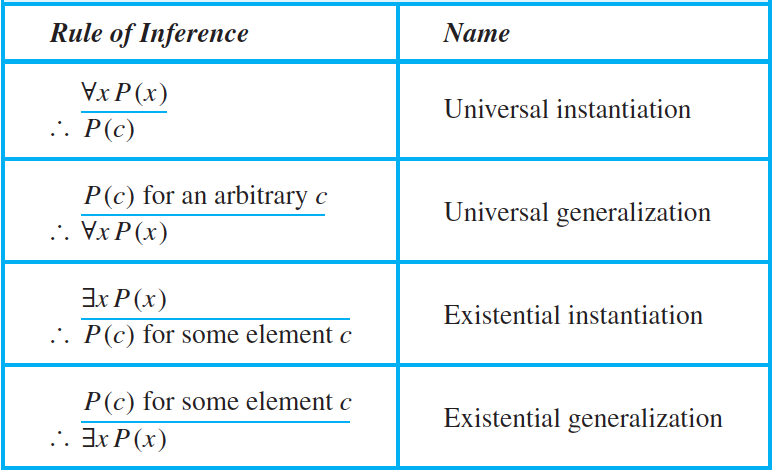
\includegraphics [width=3in]
  {Table-1-6-2-RulesOfInferenceForQuantifiedStatements}
  \caption{RulesOfInferenceForQuantifiedStatements}
  \label{table:RulesOfInferenceForQuantifiedStatements}
  \end{table}
  
   \subsection {Combining Rules of Inference for Propositions and Quantified Statements}
Here is one example of how the rules of inference for propositional logic can be applied with rules of inference for quantified statements as well. 

Given:
For all positive integers $n$, if $n$ is greater than 4, then $n^2$ is less than $2^n$,
Prove:
$$100^2 < 2^{100}$$


One inference rule that uses both propositional and predicate logic is \textbf{universal modus ponens}. This rule tells us that if $\forall x(P(x) \rightarrow Q(x))$ is true, and if $P(a)$ is true where $a$ is some specific member of the domain, then $Q(a)$ will also be true. Here is an example:

\begin{example}
Given that for all positive integers $n$, if $n$ is greater than 4, then $n^2$ is less than $2^n$, prove that $100^2 < 2^{100}$.
\begin{proof}
Let $P(n)$ denote "$n>4$" and let $Q(n)$ denote "$n^2$". The statement "For all positive integers $n$, if $n$ is greater than 4, then $n^2$ is less than $2^n$ can be represented by $\forall n(P(n) \rightarrow Q(n)$, where the domain consists of all positive integers. We start by assuming that $\forall n(P(n) \rightarrow Q(n)$ is true. Note that $P(100)$ is true because $100 > 4$. It follows by universal modus ponens that $Q(n)$ is true, namely that $100^2 < 2^{100}$. 
\end{proof}
 \end{example}
 
Note that this proof proceeded from its premises to its conclusion by applying one rule of inference or logic sequentially until the conclusion was affirmed. This is an example of a \textbf{Direct Proof}. Here is another example.

\begin{example}
Prove that if $n$ is an odd integer, then $n^2$ must be odd.
\begin{proof}
Note that this problem states $\forall n (P(n) \rightarrow Q(n))$, where "$P(n)$ is an odd integer" and "$Q(n)$ is $n^2$ is odd". The proof procedes by proving the implication. We begin the proof by assuming the antecedent of the implicaiton, that $P(n)$ is true and that $n$ is an odd integer. By the definition of an odd integer we have $\exists k : n=2k+1$, where $k$ is an integer. If we square both sides of the equation $n=2k+1$ we get $n^2=(2k+1)^2$ which gives us $4k^2+4k+1$. Factoring out 2 gives us $2(2k^2+2k) + 1$. We know that $k$ is an integer, that squaring an integer gives us an integer and that $2k$ will also be an integer and that adding an integer to an integer gives us an integer. Therefore we know that $(2k^2+2k)$ is an integer. This shows that the right side of the equation has the form twice some integer plus one which we know to satisfy the defintion of what it means to be odd. This proves that $n^2$ must be an integer satisfying the proof obligation to show that squaring an odd number must necessarily give us an odd integer. 
\end{proof}
\end{example}

There are times when the attempt to perform a direct proof  of an implication seems to lead to a dead end. When this happens it is sometimes easier to prove the contrapositive of the implication. This form of proof is called \textbf{Proof by Contraposition} as we demonstrate here:

\begin{example}
Prove that if $n$ is an integer and $3n+2$ is odd, then $n$ is odd.
\begin{proof}
We might proceed with the usual practice of assuming the antecedent and trying to derive the conclusion. This gives us that $3n+2$ is odd which means that $3n+2 = k+1$ where $k$ is some integer. We want to prove that $n$ is odd but there does not seem to be an easy way to proceed. We will try proving the contraposition instead. First we must state the contrapositive of the implication which we state as, if it is not the case that $n$ is odd, then it is not the case that $3n+2$ is odd.($\neg q\rightarrow \neg p$) We can use the fact that if something is not odd it must be even and restate the contraposition as, if $n$ is even, then $3n+2$ is even. If $n$ is even it can be restated as $2k$ where $k$ is some integer. Substituting we can restate the conclusion as $3(2k)+2$ or $6k+2$. We can factor out the 2 giving $2(3k+1)$ which fits the definition of an even number proving the consequent and concluding the proof.
\end{proof}
\end{example}

\begin{example}
Prove: If pigs can fly, then I sing better than Justin Bieber.
\begin{proof}
We are asked to prove another implication. In this case the antecedent of the implication is clearly false since we know that pigs cannot fly. Recall that an implication with a false antecedent is always true. A false premise can be used to "prove" anything.
\end{proof}
\end{example}

This is an example what is called a vacuuous proof. Here is a more interesting example.

\begin{example}
Prove that if $n = ab$, where $a$ and $b$ are positive integers, then $a \le \sqrt {n}$ or $b \le \sqrt{n}$
\begin{proof}
Because there is no obvious way of showing that $a \le \sqrt{n}$ or $b \le \sqrt{n}$
 directly from the equation $n = ab$, where $a$ and $b$ are positive integers, we attempt a proof by contraposition.
The first step in a proof by contraposition is to assume that the conclusion of the conditional statement “If $n = ab$, where $a$ and $b$ are positive integers, then $a \le \sqrt{n}$ or $b \le \sqrt{n}$'' is false.  That is, we assume that the statement $(a \le \sqrt{n}) \lor (b \le \sqrt{n})$ is false. Using the meaning of disjunction
together with De Morgan’s law, we see that this implies that both $(a \le \sqrt{n})$ and $(b \le \sqrt{n})$ are false.

This implies that $a > \sqrt{n}$ and $b > \sqrt{n}$. We can multiply these inequalities together (using the fact that if $0 < s < t$ and $0 < u < v$, then $su < tv$) to obtain $ab > \sqrt{n} \dots \sqrt{n} =n$. This shows that $ab \neq n$, which contradicts the statement $n = ab$. Because the negation of the conclusion of the conditional statement implies that the hypothesis is false, the original conditional statement is true. Our proof by contraposition succeeded; we have proved that if $n = ab$, where $a$ and $b$ are positive integers, then $a \le\sqrt{n}$ or $b \le \sqrt{n}$.
\end{proof}
\end{example}


The last section introduced a great deal of terminology and basic logical structure. But many feel that real mathematics, including logic, does not begin until one begins to reason about the material and attempt to determine new truths from the truths that are either accepted as true or which can be arrived at through reason. This chapter is a fast introduction to this mode of reasoning.

The chapter introduces the basic terminology of deductive reasoning and its presentation in the form of formal proofs. Various proof methods and strategies are summarized with classic examples. The remainder of the book will build upon this basis and demonstrate good proof style.

\section {Introduction to Proofs}
  \subsection {Why Write Proofs?}
Mathematics can be distinguished from other scientists by the kind of reasoning that we do. For reasons that this course explains, computer science is mostly a form of applied mathematics and therefore learning how to do mathematical proofs is a needed skill for a true computer scientist. Reasoning is often split into two types, inductive and deductive. Inductive reasoning is that which tries to generalize from a series of observations while deductive uses logic to conclude that an assertion must be true based on other statements that are already accepted as true. When someone gives a series of assertions that each build on what has come before and using accepted reasoning, we say they have proven their assertion and that the argument is a valid proof of the assertion. This has been a part of logic since at least Euclid's geometry and continues to be a cornerstone of undergraduate education. This chapter will be a poor substitute for a full semester course on the subject but should at least prepare the student for more formal work.

  \subsection{What Am I Allowed to Assume for this Proof?}
Given the emphasis on using accepted truths as premises, the student quickly finds themselves asking, what am I allowed to assume as either a premise or a rule of inference? The last chapter gave the most common ones from logic but often the student must use some high school algebra. The simple answer is that anything you could do in high school as valid algebra can be done in a proof for this course. More formally it must be something that can be justified by some argument to authority, which will be some previously published property. And of course it needs to be applied correctly. What cannot be done is to introduce a truth that in any way assumes the conclusion one is trying to make. We deal with that in this chapter when talking about fallacies.

Some students are uncomfortable with the handwaving of allowing that which was admitted in high school math. For reasons beyond the scope of this book it is not possible to put all of arithmetic onto a firm axiomatic basis. But to help the nervous here is a brief list of high school algebra: 
\begin{itemize}
  \item Closure Laws for Addition and Multiplication
  \item Associative Laws for Addition and Multiplication
  \item Commutative Laws for Addition and Multiplication
  \item Additive and Multiplicative Identity Laws
  \item Identity Elements Axiom
  \item Inverse Laws for Addition and Multiplication
  \item Distributive Laws
  \item Trichotomy Law
  \item Transitivity Law
  \item Additive Compatibility Law
  \item Multiplicative Compatibility Law
 \end{itemize}

For this text we take one more axiom that may not always be covered in a high school class but which we will need in the section on induction. That is called the \textit{completeness property}. This includes the definition of the upper bound and least upper bound. 

\begin{definition}[Completeness Property]\label{CompletenessProperty}
Every nonempty set of real numbers that is bounded above has a least upper bound.
\end{definition}


    informal proofs, theorem, propositions, facts, results, proof, axioms, postulates, lemma, corollary, conjecture
    \subsection {Understanding How Theorems Are Stated}
Often there is an \textbf{assertion} we want to make, some \textbf{proposition} which must either be true or false. Assertions often start as \textbf{conjectures}, propositions which we do not yet know are either true or false and which we would like to have a proof but do not yet have one. We often start with basic definitions which are essentially \textbf{axioms} that we accept as true without question. We must then construct a series of statements that each make new assertions by using the prior axioms and the \textbf{accepted rules of inference}. If we are successful, the final assertion is the proposition we wanted to prove which we call the \textbf{conclusion} of the argument. When we are presenting the assertion with the list of infered assertions that lead to the conclusion, we call this a \textbf{proof}. \textbf{Theorems} are nothing more than assertions we find helpful presented with their arguments as to why the assertion must be true. 

It is not uncommon that something accepted as an axiom is later found to be untrue, that is false. Or that a proof which depended upon a prior theorem which is found to contain a flaw. This leads to an important point about proofs, one can present a \textbf{valid} argument, one which uses only valid rules of inference, yet is found to depend upon one or more premises that are false. The argument is still said to be valid but the argument unsound. To be a \textbf{sound} argument one must have valid reasoning plus true premises. 



\section{Common Argument Forms}
\subsection {Direct Proofs}
In the chapter on Logic, there was a table of logical equivalences, Table \ref{table:LogicalEquivalenceInvolvingBiconditionalStatements}. The equivalence was demonstrated by showing that no matter the truth condition of the propositions, both expressions would evaluate to the same truth value. That is, the truth tables for both columns under the expressions matched on every row. This is a proof by truth table. However the number of rows will grow exponentially with the number of propositions so this kind of proof cannot be done by hand and often not even by machine for large numbers of propositions. 

This leads to the more common style of proof which is the series of statements grounded on the prior truths but making a new and equivalent statement. We stated the rule of inference known as Modus Ponens which says that given a true conditional statement and the fact that the antecedent of the conditional is known to be true, that the consequent of the conditional must be true. 

$$p \land (p \rightarrow q) \equiv q  \text{    (Modus Ponens)}$$
    
    
  \subsection {Direct Proofs}
\begin {theorem}
The sum of two even numbers is even
\begin{proof}[Two-Column Formal]
Let n,m be the two even numbers (premise given)\\
Then n=2*k and m=2*j where k and j are integers (def of even)\\
Then n+m=2*k + 2*j (basic law of arithmetic)\\
Then n+m=2*(k+j) (associative law of arithmetic)\\
Then n+m is even (def of even)   \\
\end{proof}
\end{theorem}

\begin{theorem}
The sum of two even numbers is even.
\begin{proof}[Prose Style]
Let $a$ and $b$ be the two even integers. We know by the definition of even that both can be expressed as twice two other integers $c$ and $d$ such that $a=2c$ and $b=2d$. Then the sum of $a+b$ can be expressed as $2c+2d$. After factoring out  the 2 we see that the sum fits the definition of even.
\end{proof}
\end {theorem}


    \subsection {Proof by Contraposition}\index{proof by contraposition}
    indirect proofs, vacuous and trivial proofs
    \subsection {Proofs by Contradiction}\index{proof by contradiction} 
    A proposition must be either true or false (rule of excluded middle). If it can be shown that a proposition cannot be false, then it must be true. To do this assume the opposite of what is to be proven and then show that it leads to a contradiction. Recall that a contradiction is false regardless of the truth values of the propositions. Once this is done you can assert that the contradiction is false and then conclude that the hypothesis must be true.
    \subsection {Exhaustive Proof and Proof by Cases}
    without loss of generality (WLOG)
    \subsection {Mistakes in Proofs}
    begging the question, circular reasoning


    
    

    \subsection {Looking for Counterexamples}
    \subsection {Proof Strategy in Action}
    \subsection {Additional Proof Methods}


\section{Proof Styles}
  \subsection{Proof by Truth Table}
If you can show that two statements always have the same truth value regardless of the truth value of the variables in the expression, you have demonstrated logical equivalence and one can always be substituted for the other where ever it appears. This can be done by creating a truth table with each expression at the top of a column and a row for every combination of truth values of the atomic propositions and show that the two columns have the same values on every row. But since the number of rows in a truth table grows exponentially with the number of atomic propositions, this method is only useful for small equivalences.
  \subsection{Two-Column Proofs}
High-school geometry teaches a two-column method. Some algebra classes use a similar approach to evaluating algebraic expressions. Most introductions to proofs begin with this form of proof presentation. Each line is a statement that is derived deductively from the lines above it. This is less tedious than a truth table proof and seems to correspond with how humans can follow detailed logic. In the most rigorous approach each line must list the inference explicitly in the right hand column to justify the statement just made. This has the advantage of making a student carefully understand how they are using logic to make the statements and easier for a grader to see that valid logic has always been applied. But the insistence on listing every rule applied makes the proof tedious for longer proofs as trivial points of logic clutter the work.
  \subsection{Prose Style Proofs}
Traditional mathematicians used a prose style of proof. The best of this technique applies all the rules of non-fiction writing. You make reasonable assumptions of what your reader will easily follow and which leaps of inference require some parenthetic remark to aid the reader. Good proof presentations in this form use natural language in a rigorous way yet will still suffer from an occassional slip  in inference. Yet by the end of the first introduction to proofs this is the way undergrads are expected to present their proofs. The vital point to recall is that any proof in this form could be reduced to a two-column proof if demanded. Experienced graders will look for large leaps and critically examine the inference to see if it is valid. If you feel it is correct but cannot justify it to yourself, take the time to break it into two or more steps that you can see the rule application.
  \subsection{Other Proof Styles}
There is an example of proof by combinatorial argument and a couple others in this and other texts. After the student becomes comfortable with these basics of formal argumentation we believe she will be well prepared to expand her ability to learn new techniques of mounting formal arguments.

Machine proofs are an area of research and many more rigorous proof styles have been described in the past 100 years. This is beyond the scope of an introductory proof class but we mention some of the notational forms used to prepare you for more advanced work. 

Note that many proofs are presented in this fashion and will use a notation called a turnstile $\vdash$:
    
\begin{comment}
\section {Methods of Proving Theorems}
This section describes the most basic form of proof style which is the direct proof and introduces the language with which we discuss proofs.
    \subsection {Direct Proofs}
In the chapter on Logic, there was a table of logical equivalences, Table \ref{table:LogicalEquivalenceInvolvingBiconditionalStatements}. The equivalence was demonstrated by showing that no matter the truth condition of the propositions, both expressions would evaluate to the same truth value. That is, the truth tables for both columns under the expressions matched on every row. This is a proof by truth table. However the number of rows will grow exponentially with the number of propositions so this kind of proof cannot be done by hand and often not even by machine for large numbers of propositions. 

This leads to the more common style of proof which is the series of statements grounded on the prior truths but making a new and equivalent statement. We stated the rule of inference known as Modus Ponens which says that given a true conditional statement and the fact that the antecedent of the conditional is known to be true, that the consequent of the conditional must be true. 

$$p \land (p \rightarrow q) \equiv q  \text{    (Modus Ponens)}$$
    
    \subsection {Proof by Contraposition}
    indirect proofs, vacuous and trivial proofs
    \subsection {Proofs by Contradiction}
    A proposition must be either true or false (rule of excluded middle). If it can be shown that a proposition cannot be false, then it must be true. To do this assume the opposite of what is to be proven and then show that it leads to a contradiction. Recall that a contradiction is false regardless of the truth values of the propositions. Once this is done you can assert that the contradiction is false and then conclude that the hypothesis must be true.

\subsection {Indirect Proof: Proof Using Contraposition}
Many proofs can be difficult to prove directly. But sometimes they are easier to prove using the contrapositive statement of the proof. This is just one common example of what is called an indirect proof. Recall that the contrapositive is the logical equivalent of any conditional statement. If you can prove the contrapositive, you have proven the conditional.

\subsection {Indirect Proof: Proof by Contradiction}
Not all proofs are given in the form of a conditional. Sometimes it is a direct assertion. Sometimes these statements can be proven using a technique called proof by contradiction or reducto absurdum. Do not confuse this with contrapositive. A contrapositive is the proof of a conditional statement while proof by contradiction is usually not. Proof by contradiction depends upon some basic truths of logic. A proposition must be either true or false, there is no other choice. This is called the law of the excluded middle. So if you can show that a statement MUST be false, then it must be true. How do you show that a statement must be false? If the statement can be restated as a contradiction, then it is false. 

The most famous example of a proof by contradiction is that the square root of 2 is irrational. This proof requires another definition from high school algebra that we state in a more casual fashion:

\begin{definition}[An Informal Definition of  Rational Number]
A rational number is one that can be expressed as the quotient of two integers.
\end{definition}

\begin{definition}[An Informal Definition of a Rational Number in Lowest Common Terms]
A rational number is in lowest terms when the numerator and denominator have no factors in common.
\end{definition}


\begin {theorem}
The square root of 2 is irrational.
\begin{proof}[Prove by contradiction: Assume the square root of 2 is rational.]
Since the square root of 2 is rational it can be expressed as the quotient of two integers. Let us call the two integers $a$ and $b$. If we divide out all common factors between $a$ and $b$, we are left with a new quotient $c/d$ of two integers with no common factor. This gives us $\sqrt{2}=c/d$ where $c/d$ is in lowest common terms. Squaring both sides give us $2=c^2/d^2$ which gives $2(d^2)=c^2$. The value $d^2$ must have an even number of the factor 2. Since we multiply this by 2 the value of $c^2$ has an odd number of the factor 2. However since $c^2$ is a square, it too must have an even number of the factor 2. This cannot be since an even number cannot also be a odd. We have derived a contradiction. In logic something cannot be both false and true and if we derive a contradiction we must reject the assumption we made as false and affirm its opposite, in this case that the square root of two must be irrational.
\end{proof}
\end {theorem}



Using the rule of substitution, we can use the rules of equivalence to give us an algebra of propositional logic. Any equivalence rule gives us an alternative way to write the expression that preserves the truth value. Note that in a truth table any two propositions will have identical columns in a truth table. In general while a truth table can be used to show equivalence, once you have more than 4 atomic propositions proving that two expressions are equivalent is more easily done with algebra than with truth tables.

argument: a set of propositions (premises) that is asserted to result in another proposition (conclusion). We formalize this to "prove" things. We say that an argument is valid when the conclusion is true whenever all the premises are true. An argument which is not valid is said to be a fallacy. A valid argument where all the premises are true is said to be sound.

We can write this in two ways:
Let P1, P2, P3, etc be a set of axioms and let Q be the conclusion

sentential, and this is equivalent to the logical statement
$P1 ^ P2 ^ P3^ ... |- Q$
and sometimes it is written as P1, P2, P3, ... |- Q where the conjunction is understood.

or 

P1
P2
P3
(underline)
therefore Q
QED

QED is short for Quod Erat Demonstrandum which means "that which was to be demonstrated. In typeset material the QED is often replaced with a black square.

There are a set of arguments that are used so often they have been given names. For example 

p, p -> q, |- q 

is known as Modes Ponens. These common arguments are summarized in Table 1.2: Rules of Inference. Note you are always free to create a new rule of equivalence.

Modus Ponens
Modus Tolens

Proof
A proof is an argument such that it accepts a certain number of propositions (axioms) which are taken to be true and using valid rules of inference and rules of equivalence results in stating the conclusion. To be a valid proof each line in the proof must be either an axiom or it must be supported by some rule of equivalence or inference. All students begin writing proofs by exhaustively showing the rules they used in a line-by-line format. But as you become more sophisticated you are allowed to skip steps that you assume the reader can follow. However if challenged you must always be prepared to give the step-by-step explanation of the reasoning.


What Can You Assume in Writing a Proof?
Students new to the formalism of mathematics can become confused as to what logical steps do not need support. In general for this class you can assume that everything you learned in secondary school can be used without support. Within a week (for the summer session) you can begin to drop the simplest logical steps and combine them. If there is doubt that the reader (your grader) will be able to see the steps you took to get to your conclusion, it is always ok to over simplify. And if you are unsure of the steps, it is always helpful to over simplify since the grader can point to the specific step you took which was invalid.

other ways are called indirect proofs
    \subsection {Proof by Contraposition}
        \subsubsection {Vacuous and Trivial Proofs}
 
\subsection {Proof Methods and Strategy}
  \subsection {Exhaustive Proof and Proof by Cases}
  \subsection {Existence Proofs}
  \subsection {Uniqueness Proofs}
    \subsection {Mistakes in Proofs}
    begging the question, circular reasoning
    \subsection {Just a Beginning}
  
\section {Proof Methods and Strategy}
    \subsection {Exhaustive Proof and Proof by Cases}
    without loss of generality (WLOG)
    
    
    \subsection {Proof Strategies}
    \subsection {Looking for Counterexamples}
    \subsection {Proof Strategy in Action}
    \subsection {Additional Proof Methods}
\end{comment}

\subsection {Proof Strategies}
  \subsection {Looking for Counterexamples}
Any assertion using a universal quantification can be refuted by citing a single counterexample.


\section{Formal Methods}
An important application of proof techniques is found in the study of what is called formal methods which includes proofs of program correctness


  \subsection {Program Verification}A program is said to be correcrt if it produces the correct output for every possible input. A proof of correctness for a program consists of two parts. The first part shows that the correct answer is obtained if the program terminates. This part is said to establish the partial correctness of the program. The second part proves that the program always terminates. When working with proofs of program correctness we use two propositions. The first, called the pre-conditions, gives a proposition that all input values must satisfy. In addition the second proposition is called the post-condition and if the program has correctly computed the value it will evaluate to true. The pre- and post-conditions are sometimes called the initial and final assertions.

\begin{definition}
A program, or program segment, $S$ is said to be partially correct with respect to the initial assertion $p$ and the final assertion $q$ if whenever $p$ is true for the input values of $S$ and $S$ terminates, then $q$ is true for the ouptut values of $S$. The notation $p[S]q$ indicates that the program, or program segment, $S$ is partially correct with respect to the initial assertion $p$ and the final assertion $q$. The notation $p[S]q$ is known as a \textit{Hoare triple}.
\end{definition}

 {Rules of Inference}
composition rule
   {Conditional Statements}
  {Loop Invariants}
        
\newpage




